\section{Auswertung}
\label{sec:Auswertung}

%%%%%%%%%%%%%%%%%%%%%%%%%%%%%%%%%%%%%%%%%%%%%%%%%%%%%%%%%%%%%%%%%%%%%%%%%%%%%%%%%%%%%%%%%%%%%%%%%%%%%%%%%%%%%%%%%%%%%%%%%%%%%%%%%%%

\subsection{Energiekalibrierung anhand des Spektrums von $\ce{^{152}}$Europium}

Zur Energiekalibrierung des Detektors wird das Spektrum eines $\ce{^{152}}$Europium-Strahlers aufgenommen, welches in Abbildung
\ref{fig:plot1} zu sehen ist.



Dazu werden anhand der charakteristischen Peaks des Spektrums mittels linearer Regression Peakenergien $E$ [1] und mittlere 
Kanalnummern $\mu_0$ in Beziehung gesetzt.
Die Peaks werden als Gaußverteilungen der Form 

\begin{equation}
  f(x) = a \cdot \text{exp}\left( - \frac{(x-\mu_0)^2}{2\sigma^2}\right) + c
  \label{eqn:gauss}
\end{equation}

genähert. Dazu wird die Funktion \textit{scipy.optimize.curve\_fit} aus der Python-Bibliothek SkiPy verwendet.
Die den Peakenergien $E$ zugeordneten Fitparameter sind in Tabelle \ref{tab:mess1} aufgelistet.
Mit den Wertepaaren der Peakenergien $E$ und der mittleren Kanalnummer $\mu_0$ wird eine lineare Regression 
der Form

\begin{equation}
  E(\mu_0) = m \cdot \mu_0 + d
  \label{eqn:eich}
\end{equation}
  
durchgeführt, die in Abbildung \ref{fig:plot5} dargestellt ist.
Die Regressionsparameter betragen

\begin{align*}
  m &= \num{0.403}\;\frac{\si{\kilo\eV}}{\text{channel}} \\
  d &= \num{-2.68 +- 0.05}\;\text{channel} \; .
\end{align*}

\begin{figure}[H]
  \centering
  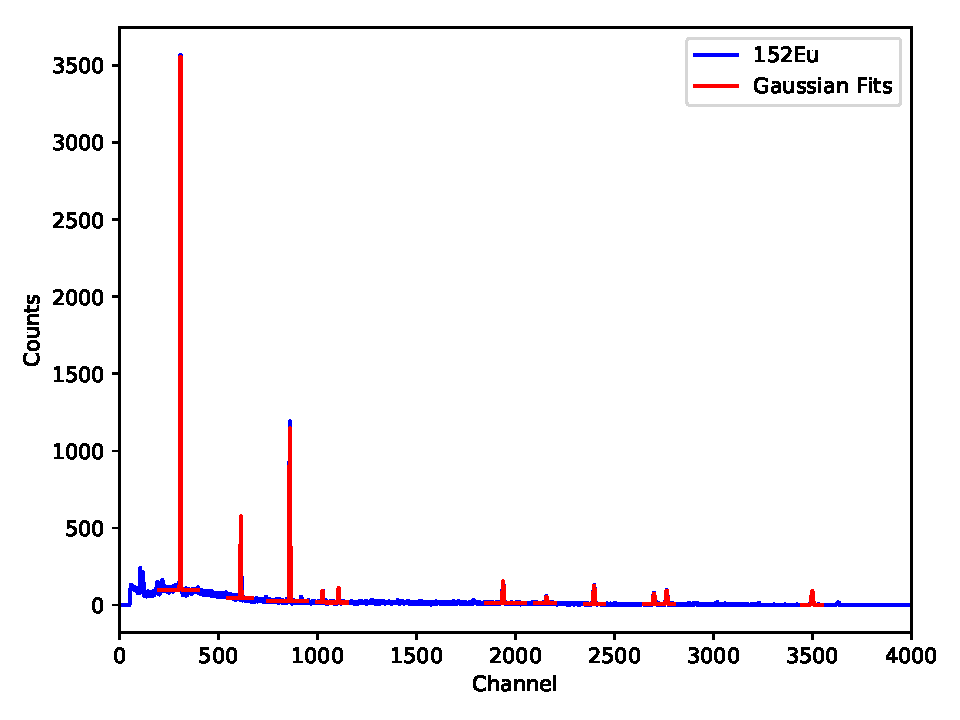
\includegraphics[scale=0.6]{content/plot1.pdf}
  \caption{Gemessenes Spektrum eines $\ce{^{152}Eu}$-Strahlers, abgeschnitten ab Kanalnummer $\num{4000}$}
  \label{fig:plot1}
\end{figure}


\begin{table}
  \small
  \centering
  \caption{Gefittete Parameter der Gaußnäherungen der charakteristischen Peaks des $\ce{^{152}Eu}$-Spektrums}
  \label{tab:mess1}
  \sisetup{table-format=2.1}
  \begin{tabular}{c c c c c}
  \toprule
  $ E \;/\; \si{\kilo\eV}$ & $\mu_0 \;/\; \text{channel}$ & $a \;/\; \text{channel}$ & $2\sigma^2 \;/\; \text{channel}^2$ & $c \;/\; \text{channel}$ \\
  \midrule
        121,78 &  308,804 $\pm$ 0,006 & 3493,0 $\pm$ 15,0 &  3,53 $\pm$ 0,04 & 100,3 $\pm$ 1,3 \\
        244,70 &  613,798 $\pm$ 0,027 &  535,0 $\pm$  9,0 &  4,15 $\pm$ 0,16 &  45,6 $\pm$ 1,1 \\
        344,30 &  860,70  $\pm$ 0,01  & 1140,0 $\pm$  6,0 &  5,51 $\pm$ 0,07 &  24,4 $\pm$ 0,6 \\
        411,12 & 1026,51  $\pm$ 0,09  &   74,7 $\pm$  3,5 &  5,7  $\pm$ 0,6  &  18,9 $\pm$ 0,8 \\
        443,96 & 1107,93  $\pm$ 0,06  &   94,2 $\pm$  3,0 &  6,4  $\pm$ 0,5  &  16,7 $\pm$ 0,5 \\
        778,90 & 1938,62  $\pm$ 0,05  &  143,3 $\pm$  2,4 & 14,3  $\pm$ 0,5  &  11,7 $\pm$ 0,4 \\
        867,37 & 2158,39  $\pm$ 0,17  &   42,5 $\pm$  2,1 & 17,1  $\pm$ 2,0  &  10,7 $\pm$ 0,4 \\
        964,08 & 2398,18  $\pm$ 0,06  &  120,3 $\pm$  2,2 & 19,3  $\pm$ 0,8  &   6,4 $\pm$ 0,5 \\
       1085,90 & 2700,41  $\pm$ 0,14  &   67,5 $\pm$  2,2 & 30,2  $\pm$ 2,3  &   5,3 $\pm$ 0,5 \\
       1112,10 & 2765,02  $\pm$ 0,11  &   88,5 $\pm$  2,6 & 23,2  $\pm$ 1,7  &   5,6 $\pm$ 0,9 \\
       1408,00 & 3499,69  $\pm$ 0,07  &   90,7 $\pm$  1,4 & 28,9  $\pm$ 1,1  &   0,9 $\pm$ 0,4 \\
  \bottomrule
  \end{tabular}
  \end{table}

\begin{figure}[H]
  \centering
  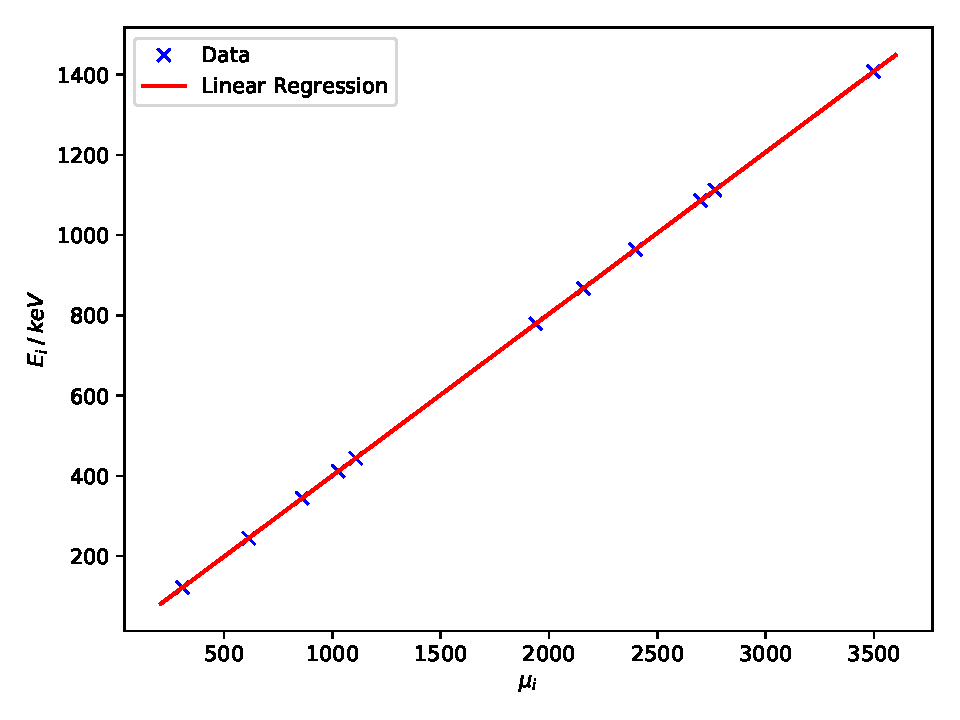
\includegraphics[scale=0.6]{content/plot5.pdf}
  \caption{Lineare Regression der Energie-Kanalnummer-Wertepaare des $\ce{^{152}Eu}$-Strahlers}
  \label{fig:plot5}
\end{figure}


%%%%%%%%%%%%%%%%%%%%%%%%%%%%%%%%%%%%%%%%%%%%%%%%%%%%%%%%%%%%%%%%%%%%%%%%%%%%%%%%%%%%%%%%%%%%%%%%%%%%%%%%%%%%%%%%%%%%%%%%%%%%%%%%%

\subsection{Bestimmung der Effizienz bzw. Vollenergienachweiswahrscheinlichkeit anhand des Spektrums von $\ce{^{152}}$Europium}

Die Effizienz

\begin{equation}
  Q = \frac{4 \pi Z}{\Omega A W t_m}
  \label{eqn:akt}
\end{equation}

wird aus der Zählrate  $Z$, dem Raumwinkel $\Omega$, der Aktivität $A$ des Strahlers, 
der Emmisionswahrscheinlichkeit $W$ und der Messzeit $t_m = \SI{4111}{\second}$ bestimmt.

Der Raumwinkel ergibt sich zu 

\begin{equation}
  \Omega = 2 \pi \left(1 - \frac{l}{\sqrt{l^2 + r^2}}\right) \approx \num{0.0538} \pi \; ,
\end{equation} 

mit dem Radius $r = \SI{2.25}{\centi\meter}$ und dem Abstand $l = \SI{9.5}{\centi\meter}$ zwischen Probe und Detektor.

Die Aktivität am Messtag wird bestimmt als

\begin{equation}
  A(t) = A_0 \cdot \text{exp} \left(- \frac{\text{ln}(2)}{t_{\sfrac{1}{2}}} \cdot t \right)  \; .
\end{equation}

Mit einer Anfangsaktivität $A_0 = \SI{4130 +- 60}{\becquerel}$ am 01.10.2000 und der Halbwertszeit
$t_{\sfrac{1}{2}} = \SI{4943 +- 5}{\day}$ ergibt sich nach einer Zeit von $t_\text{d} = \SI{6877}{\day}$
am 31.07.2019 eine Aktivität von $A(t_\text{d}) = \SI{1574 +- 23}{\becquerel}$.
Der statistische Fehler von $A(t_\text{d})$ ergibt sich nach 
Gaußscher Fehlerfortpflanzung aus denen von $A_0$ und $t_{\sfrac{1}{2}}$.

Zuletzt sind noch die Zählraten $Z$ der Peaks zu bestimmen. Dazu werden die gefitteten Gaußnäherungen integriert. 
Der konstante Parameter $2\sigma^2$ wird dabei vernachlässigt, da er das Niveau des umgebenden Spektrums angibt und somit nicht zur 
Zählrate $Z$ des Peaks beiträgt. Aus der Integration folgt dann

\begin{equation}
  Z = \int_{-\infty}^\infty \; a \cdot \text{exp}\left( - \frac{(x-\mu_0)^2}{2\sigma^2}\right) \; \text{d}x = a \sqrt{2\sigma^2\pi} \; .
  \label{eqn:rate}
\end{equation}

Der statistische Fehler der Zählrate wird aufgrund des poissonverteilten Zerfallswahrscheinlichkeit als $\sqrt{Z}$ angenommen.

In der erweiterten Tabelle \ref{tab:mess2} sind die errechneten Effizienzen $Q$, Zählraten $Z$ und 
Emmisionswahrscheinlichkeiten $W$ [1] aufgeführt.

Um eine Potenzfunktion mit Zusammenhang zwischen Effizienz und Energie zu bestimmen,
wird ein Fit einer Potenzfunktion der Form

\begin{equation}
    Q(E) = n \cdot (\frac{E}{\SI{1}{\kilo\eV}})^e
\end{equation}

durchgeführt, die in Abbildung \ref{fig:plot6} dargestellt ist.
Dazu wird die Funktion \textit{scipy.optimize.curve\_fit} aus der Python-Bibliothek SkiPy genutzt.

Es ergeben sich die Fitparameter

\begin{align*}
  n &= \num{29.37 +- 4.82} \\
  e &= \num{-0.86 +- 0.03} \; 
\end{align*}

und somit der Zusammenhang

\begin{equation}
  \label{eqn:eff}
  Q(E) \approx \num{29.37} \cdot (\frac{E}{\SI{1}{\kilo\eV}})^{\num{-0.86}} \; .
\end{equation}

\begin{table}
  \small
  \centering
  \caption{Effizienzen und zu deren Berechnung notwendige Größen des $\ce{^{152}Eu}$-Strahlers}
  \label{tab:mess2}
  \sisetup{table-format=2.1}
  \begin{tabular}{c c c c c c}
  \toprule
  $E \;/\; \si{\kilo\eV}$ & $W \;\text{in}\; \si{\percent}$ & $a \;/\; \text{channel}$ & $2\sigma^2 \;/\; \text{channel}^2$ 
  & $Z$ & $Q$ \\
  \midrule
        121,78 & 28,6 & 3493,0 $\pm$ 15,0 &  3,53 $\pm$ 0,04 & 11583 $\pm$ 108 & 0,465  $\pm$ 0,007 \\
        244,70 &  7,6 &  535,0 $\pm$  9,0 &  4,15 $\pm$ 0,16 &  1943 $\pm$  44 & 0,29   $\pm$ 0,01  \\
        344,30 & 26,5 & 1140,0 $\pm$  6,0 &  5,51 $\pm$ 0,07 &  4739 $\pm$  69 & 0,205  $\pm$ 0,004 \\
        411,12 &  2,2 &   74,7 $\pm$  3,5 &  5,7  $\pm$ 0,6  &   316 $\pm$  18 & 0,165  $\pm$ 0,012 \\
        443,96 &  3,1 &   94,2 $\pm$  3,0 &  6,4  $\pm$ 0,5  &   422 $\pm$  21 & 0,157  $\pm$ 0,009 \\
        778,90 & 12,9 &  143,3 $\pm$  2,4 & 14,3  $\pm$ 0,5  &   960 $\pm$  31 & 0,0856 $\pm$ 0,0025\\
        867,37 &  4,2 &   42,5 $\pm$  2,1 & 17,1  $\pm$ 2,0  &   312 $\pm$  18 & 0,085  $\pm$ 0,007 \\
        964,08 & 14,6 &  120,3 $\pm$  2,2 & 19,3  $\pm$ 0,8  &   937 $\pm$  31 & 0,0737 $\pm$ 0,0024\\
       1085,90 & 10,2 &   67,5 $\pm$  2,2 & 30,2  $\pm$ 2,3  &   657 $\pm$  26 & 0,074  $\pm$ 0,004 \\
       1112,10 & 13,6 &   88,5 $\pm$  2,6 & 23,2  $\pm$ 1,7  &   756 $\pm$  28 & 0,064  $\pm$ 0,003 \\
       1408,00 & 21,0 &   90,7 $\pm$  1,4 & 28,9  $\pm$ 1,1  &   864 $\pm$  30 & 0,0473 $\pm$ 0,0014\\
  \bottomrule
  \end{tabular}
  \end{table}


\begin{figure}[H]
  \centering
  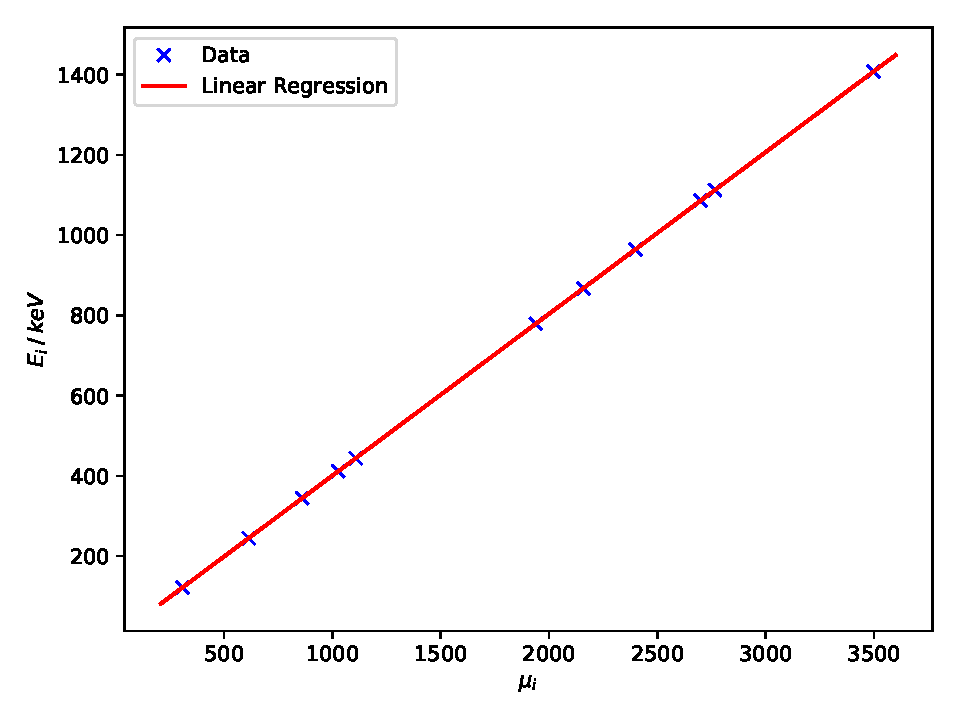
\includegraphics[scale=0.6]{content/plot6.pdf}
  \caption{Gefittete Potenzfunktion der Güte in Abhängigkeit der Energie}
  \label{fig:plot6}
\end{figure}

%%%%%%%%%%%%%%%%%%%%%%%%%%%%%%%%%%%%%%%%%%%%%%%%%%%%%%%%%%%%%%%%%%%%%%%%%%%%%%%%%%%%%%%%%%%%%%%%%%%%%%%%%%%%%%%%%%%%%%%%%%%%%%%%%%%%%%%%%%%%%

\subsection{Untersuchung des monochromatischen Gammaspektrums von $\ce{^{137}}$Caesium}

Das gemessene Spektrum von $\ce{^{137}}$Caesium ist in den Abbildungen \ref{fig:plot2} und \ref{fig:plot21} dargestellt.
Um die Lage des Photopeaks bzw. der Vollenergielinie zu bestimmen, wird dieser durch eine Gaußglocke genähert, die in Abbildung
\ref{fig:plot22} dargestellt ist.

Die Näherung erfolgt mittels der Funktion \textit{scipy.optimize.curve\_fit} aus der Python-Bibliothek SkiPy und für
das Maximum der Gaußglocke ergibt sich die Kanalnummer

\begin{equation*}
  \mu_{0,\text{Photo}} = \num{1648 +- 1} \text{channel}\; ,
\end{equation*}

die als Zentrum des Photopeaks angenommen wird.
Mit der Energie-Eichung \eqref{eqn:eich} lässt sich die Energie des Photopeaks als

\begin{equation*}
  E_\text{Photo} = \SI{661.35 +- 0.05}{\kilo\eV}
\end{equation*}

bestimmen.

\subsubsection{Halb- und Zehntelwertsbreite}

Die maximale Ereignisanzahl des gaußgenäherten Photopeaks aus Abbildung \ref{fig:plot22} beträgt $\num{1640}$.
Es lassen sich die Halb- und Zehntelwertsbreiten 

\begin{align*}
  \mu_{0, \sfrac{1}{2}} &\approx \num{5.37}\text{channel} \\
  \mu_{0, \sfrac{1}{10}} &\approx \num{10.02}\text{channel}
\end{align*} 

ablesen.

Mit der Energie-Eichung \eqref{eqn:eich} lassen sich diese in die Energienintervalle

\begin{align*}
  \Delta E_{\sfrac{1}{2}}  &= \SI{662.43 +- 0.05}{\kilo\eV} - \SI{660.27 +- 0.05}{\kilo\eV} \\
  \Delta E_{\sfrac{1}{10}} &= \SI{663.37 +- 0.05}{\kilo\eV} - \SI{659.33 +- 0.05}{\kilo\eV}
\end{align*}

umrechnen.

Dabei ist das Verhältnis zwischen Halb- und Zehntelwertsbreiten

\begin{equation}
  \kappa = \frac{\mu_{0, \sfrac{1}{10}}}{\mu_{0, \sfrac{1}{2}}} = \num{1.866}\; .
\end{equation}

Zum Vergleich mit der gemessenen kann die Halbwertsbreite der Gaußverteilung wie folgt genähert und berechnet werden:

\begin{align}
  \Delta E_{\sfrac{1}{2}, \text{theo}} &= \sqrt{8 \cdot \text{ln}(2)} \cdot \sigma \approx \num{2.35} \cdot \sqrt{F E_\text{Photo} E_\text{Ex}} \\
  &= \num{2.35} \cdot \sqrt{\num{0.1}\cdot \SI{661.35 +- 0.05}{\kilo\eV} \cdot \SI{2.9}{\eV}} = \SI{1029.16 +- 0.04}{\eV} \; .
\end{align}

Dabei beschreibt $\sigma$ die Standardabweichung der Gaußverteilung und $E_\text{Ex}$ die
Bildungsenergie von Exzitonen (Elektron-Loch-Paare) für Germanium bei einer Temperatur von $\SI{77}{\kelvin}$. 
Der Fano-Faktor $F$ berücksichtigt, dass Fluktuationen in der Erzeugung von Exzitonen
durch Fluktuation der Anregung mit Gammaquanten ausgeglichen werden.

\subsubsection{Comptonkante und Rückstreulinie}

Die Comptonkante liegt etwa bei der Kanalnummer $\mu_{0,\text{K}} = \num{1180 +- 25}\text{channel}$ und der Rückstreupeak etwa bei
$\mu_{0, \text{R}} = \num{490 +- 25}\text{channel}$.

Dies entspricht den Energien

\begin{align*}
  E_\text{K} &= \SI{473 +- 10}{\kilo\eV} \\
  E_\text{R} &= \SI{195 +- 10}{\kilo\eV} \; .
\end{align*}

Berechnet werden können die Energien nach den Gleichungen \eqref{eqn:Compton} und \eqref{eqn:Kante} zu

\begin{align*}
  E_\text{K, theo} &= E_\text{Photo} \cdot \frac{2 \epsilon}{1 + 2 \epsilon} = \SI{477.05 +- 0.05}{\kilo\eV} \\
  E_\text{R, theo} &= \frac{E_\text{Photo}}{1 + 2 \epsilon} =\SI{184.299 +- 0.004}{\kilo\eV} \; .
\end{align*}
 

\subsubsection{Inhalte und Absorptionswahrscheinlichkeiten des Photopeaks und Comptonkontinuums}

Zur Bestimmung des Inhalte bzw. der Zählraten wird die Funktion \textit{scipy.integrate.quad} 
aus der Python-Bibliothek SkiPy verwendet.
Für den in Abbildung \ref{fig:plot22} gefitteten Photopeak ergibt das die Zählrate:

\begin{equation*}
    Z_\text{Photo} = \num{9510} \; .
\end{equation*}

Zur Bestimmung der Zählrate des durch den Rückstreupeak verfälschten Comptonkontinuums wird dieses
in Abbildung \ref{fig:klein} nach dem Klein-Nishina-Wirkungsquerschnitt in Gleichung \eqref{eqn:klein} gefittet.
Dazu wird der weitgehend unverfäschte Bereich zwischen dem Rückstreupeak und der Comptonkante mit den
Kanalnummern $\num{750}$ bis $\num{1180}$ gewählt.
Der Fitparameter ergibt sich zu

\begin{equation*}
  \sigma_{Th} = (\num{4.45 +- 0.04})\cdot 10^{-12}\si{\square\meter} \; .
\end{equation*}

Für die Comptonkante ergibt sich nach Integration des Fits von Kanalnummer $\num{0}$ bis $\num{1180}$ 
die Zählrate:

\begin{equation*}
  Z_\text{Compton} = \num{33795} \; .
\end{equation*}

Nach Gleichung \eqref{eqn:Strahl} ergibt sich für die Absorptionswahrscheinlichkeit:

\begin{equation}
  W(D) = 1 - \text{e}^{- \kappa D} \; .
\end{equation}

Der Extinktionskoeffizient $\kappa$ lässt sich für verschiedene Energien aus Abbildung \ref{fig:Ext} ablesen.
Für eine Kristalllänge von $D = \SI{4.5}{\centi\meter}$ ergeben sich dann die in Tabelle \ref{tab:mess3}
aufgelisteten Absorptionswahrscheinlichkeiten.


\begin{figure}[H]
  \centering
  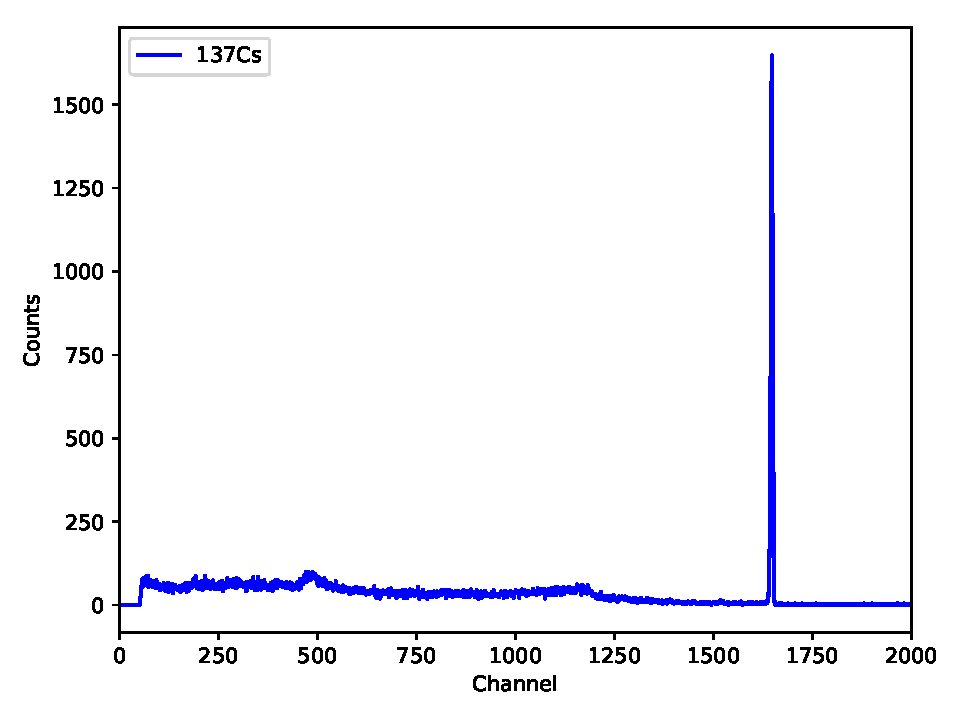
\includegraphics[scale=0.55]{content/plot2.pdf}
  \caption{Gemessenes Spektrum eines $\ce{^{137}Cs}$-Strahlers, abgeschnitten ab Kanalnummer $\num{2000}$. Hier ist der
  Photopeak bzw. die Vollenergielinie gut zu erkennen.}
  \label{fig:plot2}
\end{figure}

\begin{figure}[H]
  \centering
  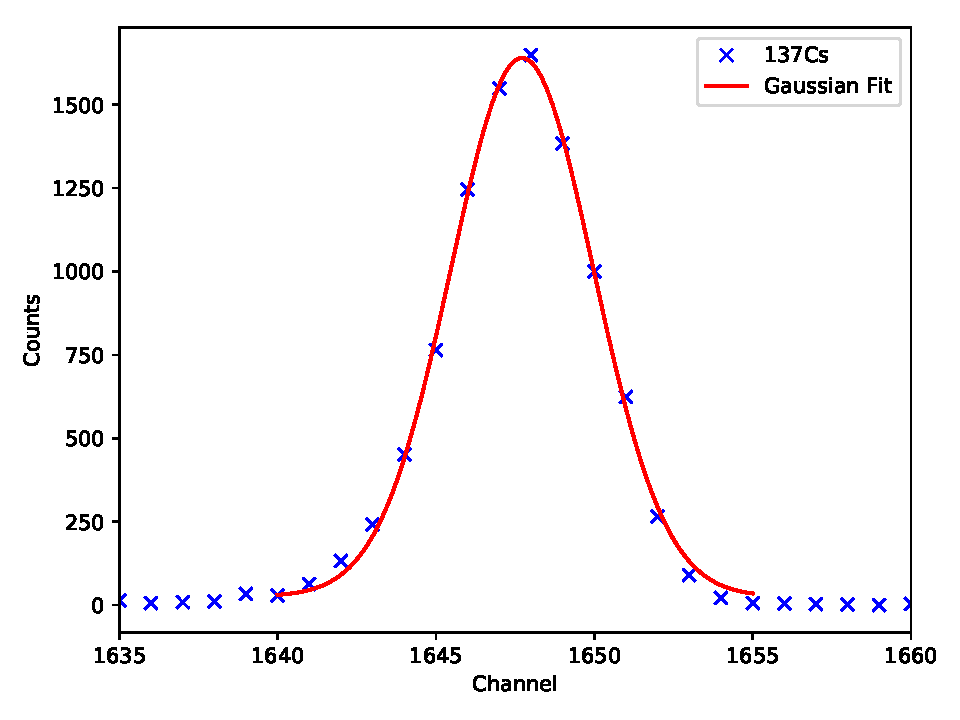
\includegraphics[scale=0.6]{content/plot22.pdf}
  \caption{Gemessener und gaußgenäherter Photopeak eines $\ce{^{137}Cs}$-Strahlers}
  \label{fig:plot22}
\end{figure}

\begin{figure}[H]
  \centering
  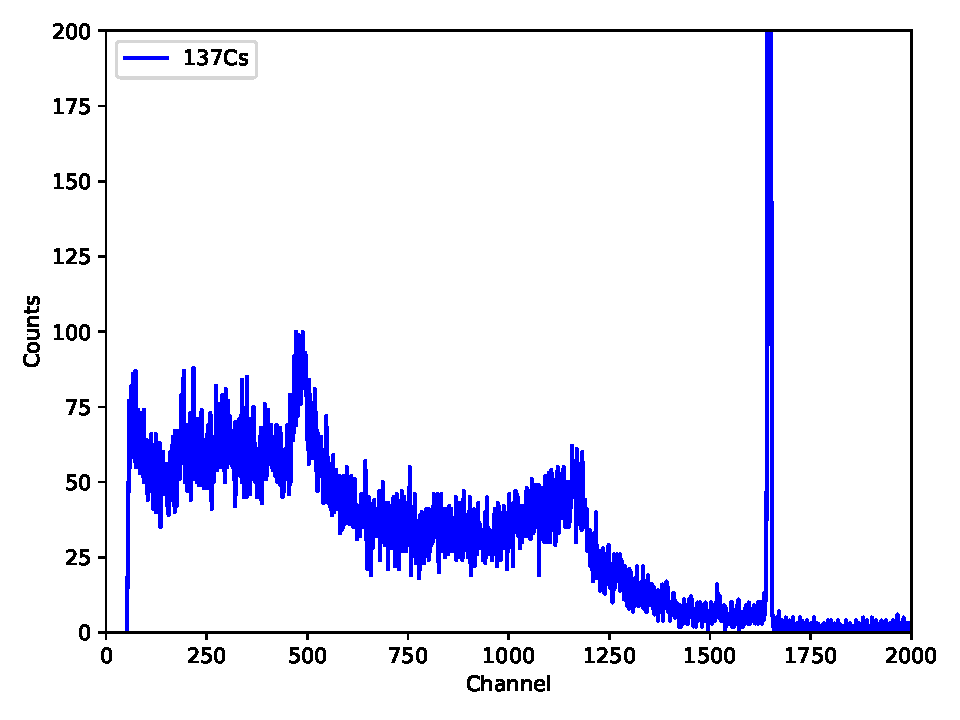
\includegraphics[scale=0.6]{content/plot21.pdf}
  \caption{Gemessenes Spektrum eines $\ce{^{137}Cs}$-Strahlers, abgeschnitten ab Kanalnummer $\num{2000}$. Zur Erkennung
    des Compton-Kontinuums, des Rückstreupeaks und der Compton-Kante wurde ein kleinerer Bereich der Ereignisanzahl gewählt.}
  \label{fig:plot21}
\end{figure}

\begin{figure}[H]
  \centering
  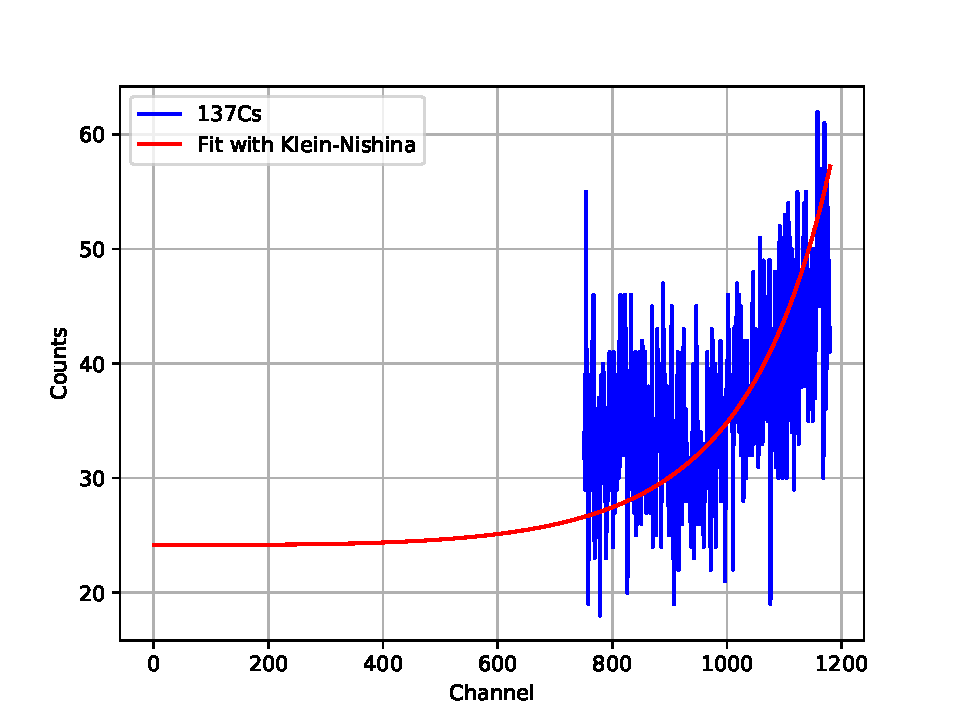
\includegraphics[scale=0.6]{content/kleinnishina.pdf}
  \caption{Gemessene Comptonkante eines $\ce{^{137}Cs}$-Strahlers von Kanalnummer $\num{750}$ bis $\num{1180}$,
  gefittet nach dem Klein-Nishina-Wirkungsquerschnitt \eqref{eqn:klein}}
  \label{fig:klein}
\end{figure}

\begin{table}
  \centering
  \caption{Energien, Extinktionskoeffizienten und Absorptionswahrscheinlichkeiten für den Photo- und Comtoneffekt des $\ce{^{152}Eu}$-Strahlers}
  \label{tab:mess3}
  \sisetup{table-format=2.1}
  \begin{tabular}{c c c }
  \toprule
  $ $ & $\text{Photoeffekt}$ & $\text{Comptoneffekt}$ \\
  \midrule
  $E \;/\; \si{\kilo\eV}$                 & 661,35 & 661,35 \\
  $\kappa \;/\; \frac{1}{\si{\centi\meter}}$ & 0,006  & 0,4    \\
  $W \;/\; \si{\percent}$                 & 2,66   & 83,47\\
  \bottomrule
  \end{tabular}
\end{table}


%%%%%%%%%%%%%%%%%%%%%%%%%%%%%%%%%%%%%%%%%%%%%%%%%%%%%%%%%%%%%%%%%%%%%%%%%%%%%%%%%%%%%%%%%%%%%%%%%%%%%%%%%%%%%%%%%%%%%%%%%%%%%%%%%%%

\subsection{Aktivitätsbestimmung von  $\ce{^{125}}$Antimon oder  $\ce{^{133}}$Barium }

Zur Identifikation, welches Nuklid das in Abbildung \ref{fig:plot3} abgebildete Spektrum besitzt, werden die Peaks gemäß
Gleichung \eqref{eqn:gauss} mithilfe der Funktion \textit{scipy.optimize.curve\_fit} aus der Python-Bibliothek SkiPy
gaußgenähert.

Aus den Fitparametren lassen sich nach Gleichung \eqref{eqn:eich} die Energien $E$, nach Gleichung 
\eqref{eqn:eff} die Effizienzen $Q$ und nach Gleichung \eqref{eqn:rate} die Zählraten $Z$ berechnen.

Nach Umstellung der Gleichung \eqref{eqn:akt} ergibt sich die Aktivität

\begin{equation}
  A = \frac{4 \pi Z}{\Omega Q W t_m}
\end{equation}

mit dem Raumwinkel $\Omega \approx \num{0.0538} \pi$ und einer Messzeit von $t_m = \SI{3771}{\second}$.
Diese gefitteten Parameter sind in Tabelle \ref{tab:mess4} und die errechneten Größen in Tabelle \ref{tab:mess5} aufgelistet.


\begin{figure}[H]
  \centering
  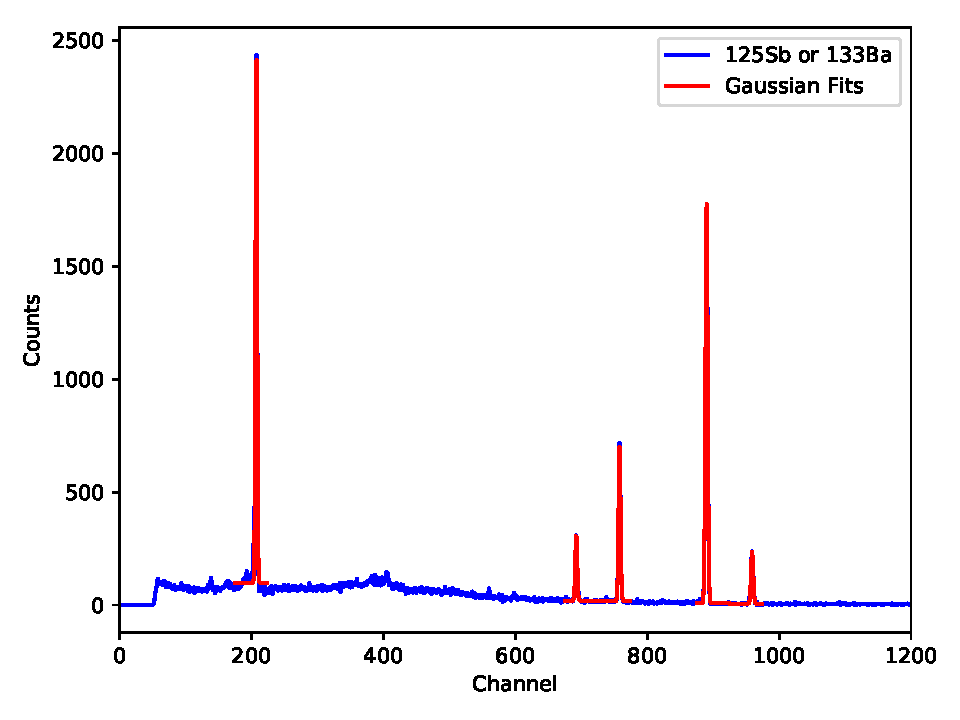
\includegraphics[scale=0.65]{content/plot3.pdf}
  \caption{Gemessenes und genähertes Spektrum eines $\ce{^{125}Sb}$- oder  $\ce{^{133}Ba}$-Strahlers,
           abgeschnitten ab Kanalnummer $\num{1200}$}
  \label{fig:plot3}
\end{figure}

\begin{table}[H]
  \centering
  \caption{Fitparameter der Gaußnäherungen des $\ce{^{125}Sb}$- oder $\ce{^{133}Ba}$-Strahlers}
  \label{tab:mess4}
  \sisetup{table-format=2.1}
  \begin{tabular}{c c c c c}
  \toprule
  $E \;/\; \si{\kilo\eV}$ & $\mu_0 \;/\; \text{channel}$ & $a \;/\; \text{channel}$ & 
  $2\sigma^2 \;/\; \text{channel}^2$ & $c \;/\; \text{channel}$ \\
  \midrule
     81,01 $\pm$ 0,05 & 207,667 $\pm$ 0,023 & 2400 $\pm$ 40 & 3,06 $\pm$ 0,11 & 99,0 $\pm$ 7,0 \\
    276,39 $\pm$ 0,05 & 692,477 $\pm$ 0,026 &  301 $\pm$  5 & 4,08 $\pm$ 0,15 & 20,0 $\pm$ 0,9 \\
    302,84 $\pm$ 0,05 & 758,120 $\pm$ 0,016 &  685 $\pm$  6 & 4,5  $\pm$ 0,1  & 17,4 $\pm$ 1,3 \\
    355,98 $\pm$ 0,05 & 889,976 $\pm$ 0,008 & 1769 $\pm$  7 & 5,46 $\pm$ 0,05 &  8,9 $\pm$ 1,6 \\
    383,82 $\pm$ 0,05 & 959,06  $\pm$ 0,04  &  231 $\pm$  4 & 5,37 $\pm$ 0,23 &  6,3 $\pm$ 0,9 \\
  \bottomrule
  \end{tabular}
\end{table}

\begin{table}[H]
  \centering
  \caption{Aktiviäten und zu deren Berechnung notwendige Größen des $\ce{^{125}Sb}$- oder $\ce{^{133}Ba}$-Strahlers}
  \label{tab:mess5}
  \sisetup{table-format=2.1}
  \begin{tabular}{c c c c c}
  \toprule
  $E \;/\; \si{\kilo\eV}$ & $W \;\text{in}\; \si{\percent}$ & $Z$ & $Q$ & $A \;/\; \si{\becquerel}$ \\
  \midrule
     81,01 $\pm$ 0,05 & 34,1 & 7440 $\pm$ 180 & 0,68 $\pm$ 0,14 &   640 $\pm$ 140  \\
    276,39 $\pm$ 0,05 &  0,5 & 1078 $\pm$  27 & 0,24 $\pm$ 0,06 & 18000 $\pm$ 4000 \\
    302,84 $\pm$ 0,05 & 18,3 & 2580 $\pm$  40 & 0,22 $\pm$ 0,05 &  1280 $\pm$ 310  \\
    355,98 $\pm$ 0,05 & 62,1 & 7330 $\pm$  40 & 0,19 $\pm$ 0,05 &  1220 $\pm$ 300  \\
    383,82 $\pm$ 0,05 &  8,9 &  949 $\pm$  26 & 0,18 $\pm$ 0,04 &  1180 $\pm$ 290  \\
  \bottomrule
  \end{tabular}
\end{table}

Aus dem Vergleich der berechneten Energien mit den Literaturwerten der Energiespektren von $\ce{^{125}}$Antimon und 
$\ce{^{133}}$Barium lässt sich erkennen, dass die gemessenen Energien einigen der Peakenergien des
$\ce{^{133}}$Barium-Spektrums entsprechen. Die Energien und Emmisionswahrscheinlichkeiten des Referenzspektrums 
sind in Tabelle \ref{tab:mess6} aufgeführt.

Zur Bestimmung der Aktivität $A$ des vorliegenden $\ce{^{133}}$Barium-Strahlers wird der Mittelwert der Aktivitäten der letzten drei
Peaks genommen, da die ersten beiden Werte stark nach unten und oben abweichen.
Die mittlere Aktivität beträgt $\bar{A} = \SI{1180 +- 383}{\becquerel}$.

\begin{table}
  \centering
  \caption{Literaturwerte der Peakenergien und Emmisionswahrscheinlichkeiten des $\ce{^{133}Ba}$-Strahlers [1]}
  \label{tab:mess6}
  \sisetup{table-format=2.1}
  \begin{tabular}{c c}
  \toprule
  $E \;/\; \si{\kilo\eV}$ & $W \;\text{in}\; \si{\percent}$ \\
  \midrule
     53,16 &  2,2 \\
     79,62 &  2,6 \\
     81,00 & 34,1 \\
    160,61 &  0,6 \\
    223,25 &  0,5 \\
    302,85 & 18,3 \\
    356,02 & 62,1 \\
    383,85 &  8,9 \\
  \bottomrule
  \end{tabular}
\end{table}

%%%%%%%%%%%%%%%%%%%%%%%%%%%%%%%%%%%%%%%%%%%%%%%%%%%%%%%%%%%%%%%%%%%%%%%%%%%%%%%%%%%%%%%%%%%%%%%%%%%%%%%%%%%%%%%%%%%%%%%%%%%%%%%%%%%%%%

\subsection{Nuklididentifikation %und Aktivitätsbestimmung 
            eines unbekannten kristallinen Strahlers}

Das vollständige Spektrum des Kristalls ist in Abbildung \ref{fig:plot41} abgebildet.



Zur Untersuchung der Peaks werden diese gemäß Gleichung \eqref{eqn:gauss} 
mithilfe der Funktion \textit{scipy.optimize.curve\_fit} aus der Python-Bibliothek SkiPy gaußgenähert.
Dies ist in Abbildung \ref{fig:plot4} zu sehen.

Die Kanalnummer $\mu_0$, Energien $E$, sowie die identifizierten Nuklide und deren Referenzenergien $E_\text{N}$[1]
sind in Tabelle \ref{tab:mess7} aufgelistet. \\

\begin{figure}
  \centering
  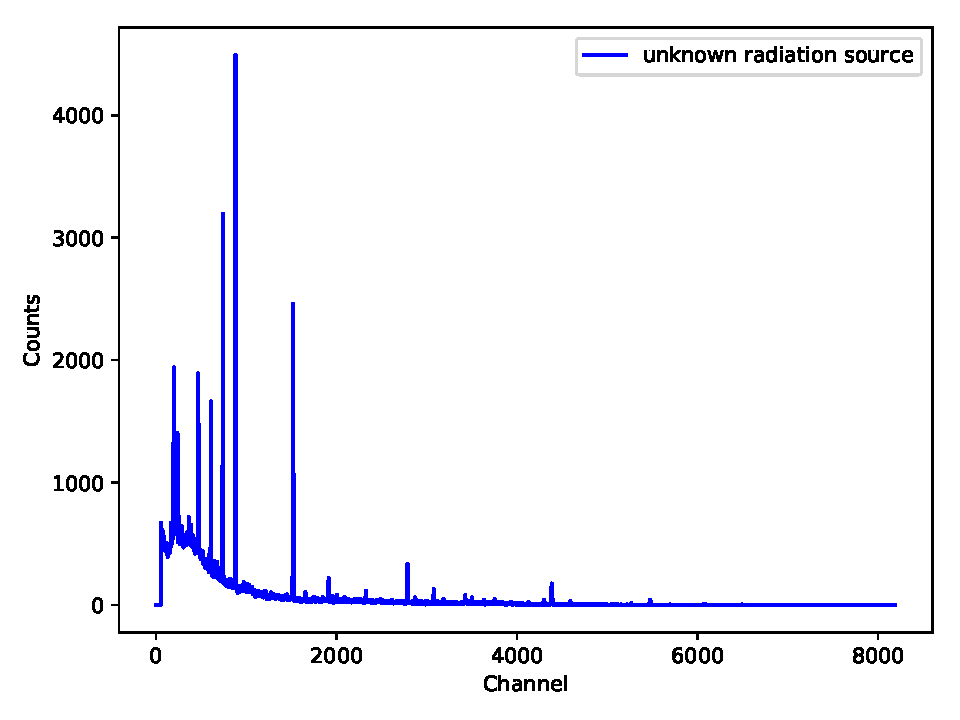
\includegraphics[scale=0.6]{content/plot41.pdf}
  \caption{Gemessenes Spektrum eines unbekannten kristallinien Strahlers}
  \label{fig:plot41}
\end{figure}

\begin{figure}
  \centering
  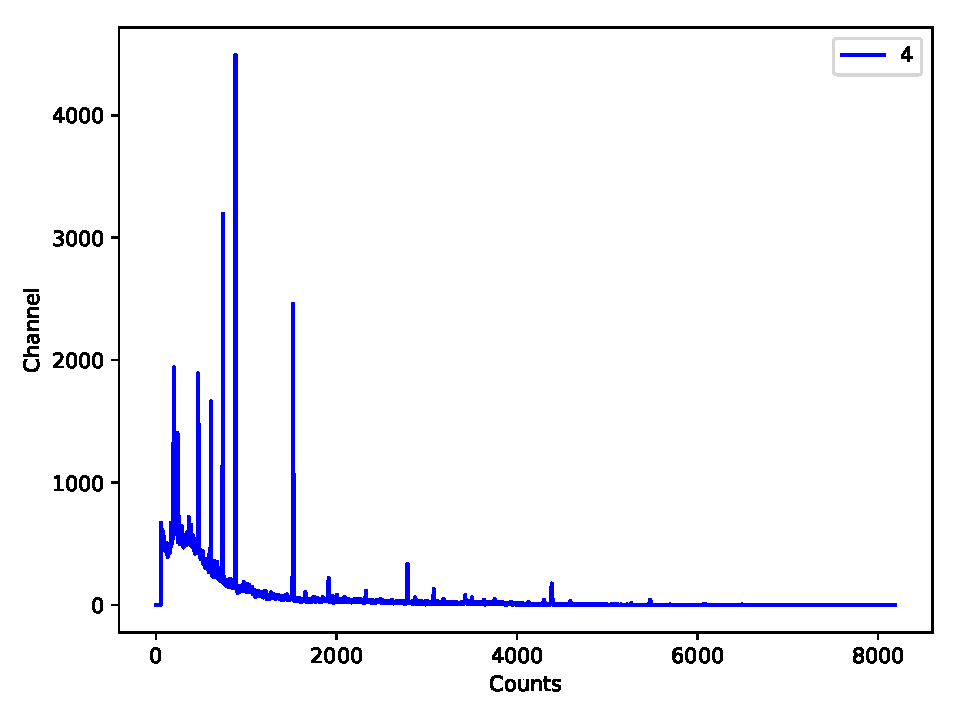
\includegraphics[scale=0.6]{content/plot4.pdf}
  \caption{Gemessenes und gaußgenähertes Spektrum eines unbekannten kristallinen Strahlers,
           abgeschnitten ab Kanalnummer $\num{6000}$}
  \label{fig:plot4} 
\end{figure}


\begin{table}
  \centering
  \caption{Fitparameter, Energien, Emmisionswahrscheinlichkeiten und identifizierte Nuklide des unbekannten Strahlers}
  \label{tab:mess7}
  \sisetup{table-format=2.1}
  \begin{tabular}{c c c c c c c}
  \toprule
  $\mu_0 \;/\; \text{channel}$ & $E \;/\; \si{\kilo\eV}$ & $E_\text{N} \;/\; \si{\kilo\eV}$ & Nuklid \\
  \midrule
   197,82 &   77,04 $\pm$ 0,05 &    - &               - \\
   237,03 &   92,84 $\pm$ 0,05 &   93 & $\ce{^{234}Th}$ \\
   468,05 &  185,94 $\pm$ 0,05 &  186 & $\ce{^{226}Ra}$ \\
   607,09 &  241,97 $\pm$ 0,05 &  242 & $\ce{^{214}Pb}$ \\
   739,04 &  295,15 $\pm$ 0,05 &  295 & $\ce{^{214}Pb}$ \\  
   879,60 &  351,80 $\pm$ 0,05 &  352 & $\ce{^{214}Pb}$ \\
  1517,94 &  609,05 $\pm$ 0,05 &  609 & $\ce{^{214}Bi}$ \\
  1656,86 &  665,03 $\pm$ 0,05 &    - &               - \\
  1912,46 &  768,04 $\pm$ 0,05 &  769 & $\ce{^{214}Bi}$ \\
  2323,78 &  933,80 $\pm$ 0,05 &  935 & $\ce{^{214}Bi}$ \\
  2785,74 & 1119,97 $\pm$ 0,05 & 1120 & $\ce{^{214}Bi}$ \\
  3077,75 & 1237,65 $\pm$ 0,05 & 1210 & $\ce{^{210}Tl}$ \\
  3424,39 & 1377,35 $\pm$ 0,05 & 1378 & $\ce{^{214}Bi}$ \\
  4384,27 & 1764,18 $\pm$ 0,05 & 1764 & $\ce{^{214}Bi}$ \\
  5475,32 & 2203,87 $\pm$ 0,05 & 2204 & $\ce{^{214}Bi}$ \\
  \bottomrule
  \end{tabular}
\end{table}


Das gemessene Spektrum weist charakteristische Linien der Nuklide
$\ce{^{234}}$Thorium, $\ce{^{226}}$Radium, $\ce{^{214}}$Plumbum (Blei), $\ce{^{214}}$Bismut und
$\ce{^{210}}$Thallium auf. Diese sind Bestandteile der Zerfallsreihe von $\ce{^{238}Uran}$.
Zwei Peakenergien können zwar keinem der Nuklide der Zerfallsreihe zugeordnet werden, dennoch kann davon ausgegangen
werden, dass es sich bei der unbekannten Strahlungsquelle um ein Urangestein handelt.
Der nicht dazu passende Peak kann entweder aus einer anderen Zerfallsreihe stammen oder es handelt sich um eine Störung
wie beispielsweise einen Rückstreupeak einer anderen Linie.


%Aus den Fitparametren lassen sich nach Gleichung \eqref{eqn:eff} die Effizienzen $Q$, nach Gleichung \eqref{eqn:rate} 
%die Zählraten $Z$ berechnen und nach Gleichung \eqref{eqn:akt} die Aktivitäten $A$ berechnen.
%Die Messzeit beträgt $t_m = \SI{4797}{\second}$ und der Raumwinkel für einen Abstand zwischen Quelle und Detektor von
%$l = \SI{1.5}{\centi\meter}$: $\Omega \approx \num{0.8906} \pi$.
%
%mit dem Raumwinkel $\Omega \approx \num{0.0538} \pi$ und einer Messzeit von $t_m = \SI{3771}{\second}$.


